\documentclass[a4paper]{article}
\usepackage[spanish,es-tabla]{babel}	% trabajar en español
\spanishsignitems	
%\usepackage{simplemargins}

%\usepackage[square]{natbib}
\usepackage{amsmath}
\usepackage{amsfonts}
\usepackage{amssymb}
\usepackage{bbold}
\usepackage{graphicx}
\usepackage{blindtext}
\usepackage{hyperref}
\usepackage{mathtools}

\begin{document}
\pagenumbering{arabic}

\Large
 \begin{center}
\textbf{Transformada Cuántica de Fourier}\\
Seminario 2  

\hspace{10pt}

% Author names and affiliations
\large
Lic. Julio A. Medina$^1$ \\

\hspace{10pt}
\small  
$^1$ Universidad de San Carlos, Escuela de Ciencias Físicas y Matemáticas\\
Maestría en Física\\
\href{mailto:julioantonio.medina@gmail.com}{julioantonio.medina@gmail.com}\\

\end{center}

\hspace{10pt}

\normalsize
La transformada de Fourier y el análisis de Fourier en general son una maquinaria matemática ubicua en la física. Esto es de esperarse ya que muchos fenómenos físicos son de naturaleza ondulatoria es decir que son fenómenos que involucran el estudio de ondas para su entendimiento, por mencionar algunos casos importantes en los que se aplica el análisis de Fourier en la física se tienen: \\

\begin{itemize}
\item Mecánica Cuántica
\item Sismología
\item Teoría electromagnética
\item Vibraciones mecánicas.
\item Procesamiento de señales naturales y artificiales.
\item Espectroscopia. 
\item Solución de ecuaciones diferenciales.
\item Teoría cuántica de campo.
\item Computación cuántica.

\end{itemize} 

\section{Transformada de Fourier Clásica}
\subsection{Series de Fourier}
Una serie de Fourier se puede definir como una expansión o una representación de una función en series de seno y coseno con la forma 
\begin{equation}\label{eq::fourier_series}
f(x)=\frac{a_0}{2}+\sum_{n=1}^\infty a_n \cos nx + \sum_{n=1}^\infty b_n \sin nx
\end{equation}
Las condiciones impuestas sobre $f(x)$ para que la ecuación anterior sea valida, son que $f(x)$ tenga un número finito de discontinuidades finitas y un número finito de valores extremos, máximos y mínimos. Estas condiciones se conocen como condiciones de Dirichlet. La teoría de Sturm-Lioville(ver \cite{Arfken}) garantiza la validez de la ecuación \ref{eq::fourier_series} usando las relaciones de ortogonalidad se pueden obtener los coeficientes de expansión
\begin{equation*}
a_n=\frac{1}{\pi} \int^{2\pi}_0 f(t) \cos{nt}\, dt
\end{equation*}

\begin{equation*}
b_n=\frac{1}{\pi} \int^{2\pi}_0 f(t) \sin{nt}\, dt, \,\,\,\,\,\, n=0,1,2,\hdots
\end{equation*}
Sustituyendo los coeficientes $a_n$ y $b_n$ en \ref{eq::fourier_series} se obtiene
\begin{equation}
\begin{aligned}
f(x)&=\frac{1}{2\pi}\int_0^\infty f(t)dt+\frac{1}{\pi}\sum_{n=1}^\infty\Big[ \cos{nx}\int_0^{2\pi} f(t) \cos{nt}\,dt + \sin{nx}\int_0^{2\pi} f(t) \sin{nt}\,dt \Big]\\
&=\frac{1}{2\pi}\int_0^\infty f(t)dt+\frac{1}{\pi}\sum^\infty_{n=1} \int^{2\pi}_0 f(t)\cos{n(x-t)\,dt}
\end{aligned}
\end{equation}
las expresiones anteriores son válidas para representar a la función $f(x)$ en el intervalo $[0,2\pi]$. Para representarlas en un intervalo de longitud $2L$ se pueden expresar la ecuación \ref{eq::fourier_series} y sus coeficientes como:
\begin{equation}
f(x)=\frac{a_0}{2}+\sum_{n=1}^\infty \Big[ a_n \cos{\frac{n\pi x}{L}} + b_n \sin{\frac{n\pi x}{L}} \Big]
\end{equation}
\begin{equation}\label{eq::Fourier_coeff}
\begin{aligned}
a_n&=\frac{1}{L} \int^{L}_{-L} f(t) \cos{\frac{n\pi t}{L}}\, dt \\
b_n&=\frac{1}{L} \int^{L}_{-L} f(t) \sin{\frac{n\pi t}{L}}\, dt, \,\,\,\,\,\, n=0,1,2,\hdots
\end{aligned}
\end{equation}
\subsection{Integral de Fourier}
Como se ha mencionado las series de Fourier son especialmente útiles para representar cierto tipo de funciones en un rango definido: $[0,2\pi]$, $[-L,L]$, y así sucesivamente como sea necesario, o en el intervalo $[-\infty,\infty]$ si la función es periódica. Ahora se analiza el problema de representar una función no periódica sobre un rango infinito. Esto se puede interpretar físicamente como la descomposición de un pulso aislado o un paquete de onda en sus componentes senoidales. Los coeficientes de la serie de Fourier en el intervalo $[-L,L]$ dados por \ref{eq::Fourier_coeff} dan cómo resultado la serie de Fourier:
\begin{equation}
\begin{aligned}
f(x)=\frac{1}{2L}\int^L_{-L} f(t)\,dt + \frac{1}{L}\sum_{n=1}^\infty \cos{\frac{n\pi x}{L}}\int^L_{-L} f(t) \cos{\frac{n\pi t}{L}}\, dt +\\
 \frac{1}{L}\sum_{n=1}^{\infty}\sin{\frac{n \pi x}{L}}\int^L_{-L} f(t)\,dt \sin\frac{n\pi x }{L}\,dt 
\end{aligned}
\end{equation}
esto se puede reescribir como 
\begin{equation}
f(x)=\frac{1}{2L}\int^L_{-L} f(t)\, dt + \frac{1}{L}\sum^\infty_{n=1}\int^L_{-L} f(t)\cos\frac{n\pi}{L}(t-x)\,dt.
\end{equation}\\
Ahora se permite que el parámetro $L$ se acerque al infinito, transformando el intervalo finito $[-L,L]$ en un intervalo infinito $(-\infty,\infty)$. Se asignan
\begin{equation}
\omega=\frac{n\pi}{L}, \,\,\,\,\,\, \Delta\omega=\frac{\pi}{L},\,\,\,\,\,\,\, \text{con } L\rightarrow\infty.
\end{equation}
Con esto se obtiene 
\begin{equation}
f(x)\rightarrow \frac{1}{\pi}\sum_{n=1}^\infty \Delta\omega \int_{-\infty}^\infty f(t) \cos{\omega(t-x)}\,dt,
\end{equation}
sustituyendo la suma infinita por una integral sobre $\omega$, se obtiene
\begin{equation}\label{eq::Fourier_integral}
f(x)=\frac{1}{\pi}\int_0^\infty\,d\omega \int_{-\infty}^\infty f(t)\cos{\omega(t-x)}\,dt,
\end{equation}
el término $a_0$ se desvanece asumiendo que $\int_{-\infty}^\infty f(t)\,dt$ existe.\\
El resultado \ref{eq::Fourier_integral} se conoce como integral de Fourier, este resultado puede expresarse convenientemente de manera exponencial al notar que 
\begin{equation}\label{eq::Fourier_cosine}
f(x)=\frac{1}{2\pi}\int_{-\infty}^{\infty}d\omega \int_{-\infty}^\infty f(t) \cos\omega(t-x)\, dt,
\end{equation}
además se tiene que 
\begin{equation}\label{eq::Fourier_sine}
\frac{1}{2\pi}\int_{-\infty}^\infty d\omega \int_{-\infty}^\infty f(t) \sin\omega(t-x)\, dt=0
\end{equation}
estos resultados son consecuencia que la función $\cos \omega (t-x)$ es una función par sobre la variable $\omega$ y $\sin\omega(t-x)$ es una función impar en $\omega$, sumando \ref{eq::Fourier_cosine} y \ref{eq::Fourier_sine} multiplicada por un factor de la unidad imaginaria $i$, se obtiene
\begin{equation}\label{eq::Fourier_exponetial}
f(x)=\frac{1}{2\pi}\int_{-\infty}^\infty e^{-i \omega x }\,d\omega \int_{-\infty}^\infty f(t)e^{i\omega t}\,dt.
\end{equation}
La variable $\omega$ es una variable arbitraria, también conocida como variable muda, juega el papel que toma un indice en una sumatoria como indice mudo, sin embargo en muchos problemas físicos $\omega$ representa una frecuencia angular. Con esto se puede interpretar a las expresiones \ref{eq::Fourier_cosine} y \ref{eq::Fourier_exponetial} como representaciones de $f(x)$ en términos de una distribución de frentes de onda de longitud infinita con frecuencia angular $\omega$ donde la frecuencia es una variable real continua.
\subsection{Transformada de Fourier}
Definiendo a una función $g(\omega)$, como la transformada de Fourier a través de 
\begin{equation}\label{eq::Fourier_trainsform}
g(\omega)\equiv \frac{1}{\sqrt{2\pi}}\int_{-\infty}^\infty f(t) e ^{i\omega t }\, dt.
\end{equation}
entonces es fácil ver que de la integral de Fourier \ref{eq::Fourier_exponetial} se tiene 
\begin{equation}\label{eq::Inverse_Fourier_transform}
f(x)=\frac{1}{\sqrt{2\pi}}\int_{-\infty}^\infty g(\omega)e^{-i \omega x}\, d\omega.
\end{equation}
esta relación también es conocida como teorema de la inversión o transformada inversa de Fourier, vale la pena notar que las expresiones \ref{eq::Fourier_trainsform} y \ref{eq::Inverse_Fourier_transform} son casi simétricas, sin embargo difieren por el signo de la unidad imaginaria $i$.
\section{Transformada Cuántica de Fourier}
\subsection{Introducción}
Como se mencionó antes la transformada de Fourier tienen mucha aplicaciones en toda la física y también tiene aplicaciones importantes en la computación clásica en áreas como el procesamiento de señales, algoritmos de compresión de datos y teoría de complejidad de algoritmos. La transformada de Fourier Cuántica es la implementación cuántica de la transformada discreta de Fourier sobre las amplitudes de una función de onda\footnote{Una función de onda que evoluciona de acuerdo a la ecuación de Schr\"{o}dinger}, es una parte fundamental de varios algoritmos cuánticos  como el algoritmo de factorización de Shor y la estimación de fase cuántica.\\
La transformada de Fourier cuántica actúa sobre un vector $(x_0, \hdots, x_{N-1})$ y lo mapea o transforma o otro vector
$(y_0, \hdots, y_{N-1})$ por medio de la siguiente fórmula
\begin{equation}
y_{k}=\frac{1}{\sqrt{N}}\sum_{j=0}^{N-1}x_j \omega_{N}^{jk}
\end{equation}
donde 
\begin{equation}\label{eq::omega_definition}
\omega_{N}^{jk}=e^{2\pi i \frac{jk}{N}}.
\end{equation}

De manera análoga la transformada cuántica de Fourier actúa sobre un estado cuántico\footnote{un vector en un espacio de Hilbert, finito o infinito} 
\begin{equation}
|X\rangle=\sum_{j=0}^{N-1} x_{j}|j\rangle
\end{equation}
y lo mapea a un estado 
\begin{equation}\label{eq::QFT_general}
|Y\rangle=\sum_{k=0}^{N-1} y_{k}|k\rangle
\end{equation}
conforme a la expresión
\begin{equation}
y_k=\frac{1}{\sqrt{N}}\sum_{j=0}^{N-1}x_j\omega_{N}^{jk}
\end{equation}
donde $\omega_{N}^{jk}$ está definido en \ref{eq::omega_definition}, es importante notar que sólo las amplitudes del estado son afectadas por está transformación, esto puede expresarse también como el mapeo
\begin{equation}
|j\rangle \rightarrow \frac{1}{\sqrt{N}}\sum^{N-1}_{k=0}\omega_N^{jk}|k\rangle
\end{equation}
o por la matriz unitaria
\begin{equation}
U_{\text{QFT}}=\frac{1}{\sqrt{N}}\sum_{j=0}^{N-1}\sum_{k=0}^{N-1}\omega_{N}^{jk}|k\rangle\langle j|
\end{equation}
\subsubsection{Intuición detrás de la TCF(QFT)}
La intuición detrás de la Transformada Cuántica de Fourier(QFT-\textit{Quantum Fourier Transform}) viene del hecho que el efecto que tiene al transformar a un estado cuántico basicamente se está cambiando de la base computacional Z  a la base de Fourier. La compuerta de Hadamard(\cite{Medina}, \cite{Qiskit}, \cite{Nielsen}) es la transformada de Fourier cuántica para un solo qubit, transforma de base computacional Z $\{|0\rangle, |1\rangle\}$ a la base X $\{|+\rangle, |-\rangle \}$. De la misma manera todos los estados de partículas múltiples es decir estados de varios qubit en la base computacional tiene una representación en la base de Fourier. La TCF simplemente es la función que transforma entre estas bases.
\begin{equation}
\text{QFT}|x\rangle = |\tilde{x}\rangle
\end{equation}
donde la base de Fourier se denota como $|\tilde{x}\rangle$.
\subsection{Ejemplo 1: TCF de 1-qubit}
Se empieza por considerar como el operador QFT definido previamente, actúa sobre  un estado de un solo qubit, i.e. $|\psi\rangle=\alpha|0\rangle+\beta |1\rangle$. Para este caso $x_0=\alpha, x_1=\beta$, y $N=2$, con esto se obtiene
que el primer coeficiente de Fourier en la transformación es 
\begin{equation}
y_0=\frac{1}{\sqrt{2}}\Bigg( \alpha \exp\bigg( 2\pi i \frac{0\times 0}{2}{•} \bigg) + \beta \exp\bigg( 2\pi i \frac{1\times 0}{2}{•} \bigg) \Bigg)=\frac{1}{\sqrt{2}}(\alpha+\beta)
\end{equation}
y para el segundo coeficiente se tiene
\begin{equation}
y_1=\frac{1}{\sqrt{2}}\Bigg( \alpha \exp\bigg( 2\pi i \frac{0\times 1}{2}{•} \bigg) + \beta \exp\bigg( 2\pi i \frac{1\times 1}{2}{•} \bigg) \Bigg)=\frac{1}{\sqrt{2}}(\alpha-\beta)
\end{equation}
con esto se obtiene el resultado total sobre $|\psi\rangle$
\begin{equation}
U_{\text{QFT}}|\psi\rangle=\frac{1}{\sqrt{2}}(\alpha+\beta)|0\rangle + \frac{1}{\sqrt{2}}(\alpha-\beta)|1\rangle
\end{equation}
está operación es equivalente a aplicar el operador de Hadamard
\begin{equation}\label{eq::Hadamard_gate}
H=\frac{1}{\sqrt{2}}
\begin{bmatrix}
1&1\\
1&-1
\end{bmatrix}
\end{equation}
al estado $\vert \psi\rangle$, 
\begin{equation}
\begin{aligned}
H\vert\psi\rangle&=\frac{1}{\sqrt{2}}(\alpha+\beta)|0\rangle + \frac{1}{\sqrt{2}}(\alpha-\beta)|1\rangle\equiv \tilde{\alpha}\vert 0\rangle+ \tilde{\beta}\vert 1\rangle\\
&=\alpha \vert + \rangle +\beta \vert - \rangle
\end{aligned}
\end{equation}
\subsection{Transformada Cuántica de Fourier: definición general}
La ejemplo anterior no deja del todo claro el como se aplica una transformada cuántica de Fourier para N más grandes. Aquí se toma a $N=2^n$, es decir $U_{\text{QFT}_N}$ actuando en el estado $|x\rangle=|x_1\hdots x_n\rangle$\footnote{Se hace uso de la notación $|x_1\hdots x_n\rangle=|x_1\rangle\otimes\hdots\otimes |x_n\rangle$ } donde $x_1$ es el bit más significativo. Con esto se aplica la expresión \ref{eq::QFT_general} para obtener
\begin{equation}\label{eq::QFT}
\begin{aligned}
U_{\text{QFT}_N}|x\rangle &=\frac{1}{\sqrt{N}}\sum_{y=0}^{N-1}\omega_N^{xy}|y\rangle\\
&=\frac{1}{\sqrt{N}}\sum_{y=0}^{N-1} e^{2\pi i xy/2^{n}}|y\rangle
\end{aligned}
\end{equation}
reescribiendo $y$ en notación fraccional binaria $y=y_1\hdots y_n$ con
\begin{equation*}
\frac{y}{2^n}=\sum_{k=1}^{n}\frac{y_k}{2^k}
\end{equation*}
donde $y_k \in\{ 0, 1 \}$, sustituyendo en \ref{eq::QFT} se obtiene
\begin{equation}\label{eq::QFT_2}
\begin{aligned}
U_{\text{QFT}_N}|x\rangle &=\frac{1}{\sqrt{N}}\sum_{y=0}^{N-1}e^{2\pi i(\sum_{k=1}^n y_k/2^k)}|y_1 \hdots y_n\rangle\\
&=\frac{1}{\sqrt{N}}\sum_{y=0}^{N-1} \prod_{k=1}^n e^{2\pi i x y_k/2^{k}}|y_1 \hdots y_n\rangle
\end{aligned}
\end{equation}
donde se ha expresado al exponencial de una suma como un producto de exponenciales. Re-arreglando las sumas y productos, y expandiendo $\sum_{y=0}^{N-1}=\sum_{y_1=0}^1 \sum_{y_2=0}^1 \hdots \sum_{y_n=0}^1$, se obtiene
\begin{equation}\label{eq::QFT_3}
\begin{aligned}
U_{\text{QFT}_N}|x\rangle &=\frac{1}{\sqrt{N}} \bigotimes_{k=1}^n \bigg(|0\rangle + e^{2\pi i x/2^k}|1\rangle \bigg)  \\
&=\frac{1}{\sqrt{N}}\bigg(|0\rangle + e^{\frac{2\pi i}{2} x} |1\rangle \bigg)\otimes\bigg(|0\rangle + e^{\frac{2\pi i}{2^2} x} |1\rangle \bigg)\otimes \hdots \otimes \bigg(|0\rangle + e^{\frac{2\pi i}{2^{n}} x} |1\rangle \bigg)
\end{aligned}
\end{equation}
\section{Circuito para la Transformada Cuántica de Fourier}
La transformada cuántica de Fourier se puede implementar utilizando el modelo de circuitos cuántico utilizado por varias implementaciones reales de la computación cuántica, para ver una introducción de estos circuitos  se puede consultar \cite{Qiskit}, \cite{Medina}, \cite{Nielsen} etc. Para construir el circuito de QFT se utilizan 2 compuertas, la primera es una compuerta de un solo qubit i.e. la compuerta de Hadamard \ref{eq::Hadamard_gate}, de la discusión del ejemplo de la QFT para 1-qubit y de la deducción de la expresión general para la QFT se sabe que para el estado de un solo qubit $\vert x_k\rangle$ la transformada de Fourier cuántica correspondiente es 
\begin{equation}
H\vert x_k\rangle=\frac{1}{\sqrt{2}}\bigg(\vert 0\rangle + \exp{\bigg(\frac{2\pi i}{2} x_k}\bigg)\vert 1\rangle\bigg)
\end{equation}
la segunda compuerta para 2 qubit, es la rotación controlada $C\,\text{ROT}_k$, que en notación de bloques de matrices está definida como 
\begin{equation}
C\,\text{ROT}_k=
\begin{bmatrix}
\mathbf{I}& 0\\
0& U\,\text{ROT}_k\\
\end{bmatrix}
\end{equation}
donde 
\begin{equation}
U\,\text{ROT}_k=
\begin{bmatrix}
1& 0\\
0& \exp{\big(\frac{2\pi i}{2^k}\big)}\\
\end{bmatrix}
\end{equation}
El efecto de aplicar $C\,\text{ROT}_k$ en un estado de dos qubits $\vert x_l x_j\rangle$ donde el primer qubit es el qubit de control y el segundo qubit es el objetivo, viene dado por
\begin{equation}
C\,\text{ROT}_k \vert 0\,x_j\rangle=\vert 0 \, x_j\rangle
\end{equation}
y
\begin{equation}
C\,\text{ROT}_k \vert 1\,x_j\rangle=\exp{\bigg(\frac{2\pi i }{2^k} x_j\bigg)}\vert 1 \, x_j\rangle
\end{equation}
Con estas dos compuertas se puede construir el circuito que implementa la transformada de cuántica de Fourier como se muestra en el siguiente diagrama\\

\begin{figure}[h]
\begin{center}
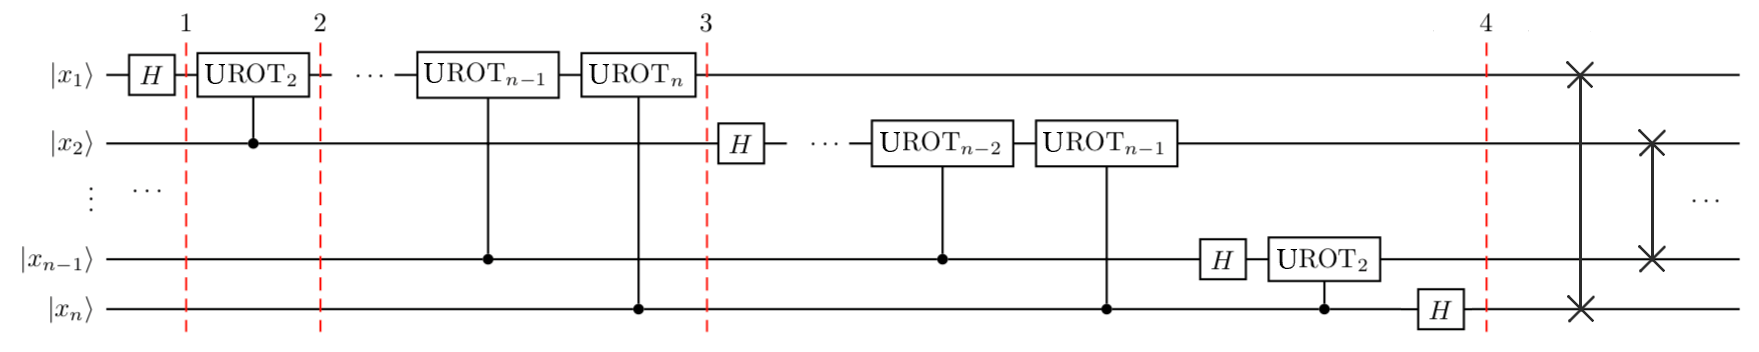
\includegraphics[scale=0.29]{./qft_circuit.png} 
\end{center} 
\caption{Implementación de circuito QFT}
\label{fig::QFT_circuit}
\end{figure}
El circuito opera de la siguiente manera. Se empieza con un estado de entrada $\vert x_1\, x_2\hdots x_n\rangle$.
\begin{enumerate}
\item Se aplica la compuerta de Hadamard al primer qubit y se transforma al estado de entrada de la siguiente manera
\begin{equation}
H_1\vert x_1 x_2\hdots x_n\rangle=\frac{1}{\sqrt{2}}\bigg[\vert 0\rangle + \exp{\bigg(\frac{2\pi i }{2} x_1\bigg)}\vert 1\rangle\bigg] \otimes \vert x_2 x_3\hdots x_n\rangle
\end{equation}
\item Después se aplica la compuerta $U\,\text{ROT}_2$ al qubit 1 controlado por el qubit 2, esto resulta en 
\begin{equation}
\frac{1}{\sqrt{2}}\bigg[\vert 0\rangle + \exp{\bigg(\frac{2\pi i }{2^2} x_2+\frac{2\pi i }{2} x_1\bigg)}\vert 1\rangle\bigg] \otimes \vert x_2 x_3\hdots x_n\rangle
\end{equation}
\item Este proceso del paso anterior se repite hasta llegar al qubit n, es decir cuando se aplica la última compuerta $U\,\text{ROT}_n$ al qubit 1 controlado por el qubit $n$, el estado es transformado a
\begin{equation}\label{eq::step3_QFT_circuit}
\frac{1}{\sqrt{2}}\bigg[\vert 0\rangle + \exp{\bigg(\frac{2\pi i }{2^n} x_n+\frac{2\pi i }{2^{n-1}} x_{n-1}+\hdots +\frac{2\pi i }{2^2} x_2+\frac{2\pi i }{2} x_1\bigg)}\vert 1\rangle\bigg] \otimes \vert x_2 x_3\hdots x_n\rangle
\end{equation}

Notando que\footnote{Se hace la observación que al final $x$ es una etiqueta para el estado y $\{x_1,\hdots,x_n\}\in \{0,1\}$, por lo que se tiene es una representación de la etiqueta de forma binaria, i.e. base 2}
\begin{equation}
x=2^{n-1} x_{1}+2^{n-2} x_{2}+\hdots+ 2^{1} x_{n-1}+2^{0} x_{n}
\end{equation}
se puede escribir el estado \ref{eq::step3_QFT_circuit} como 
\begin{equation}
\frac{1}{\sqrt{2}}\bigg[\vert 0\rangle + \exp{\bigg(\frac{2\pi i }{2^n} x\bigg)}\vert 1\rangle\bigg] \otimes \vert x_2 x_3\hdots x_n\rangle
\end{equation}
\item Después de una secuencia análoga a la de los pasos 1-3 para los qubits $2\hdots n$ se obtiene el estado final
\begin{equation}
\begin{aligned}
\frac{1}{\sqrt{2}}\bigg[\vert 0\rangle + \exp{\bigg(\frac{2\pi i }{2^n} x\bigg)}\vert 1\rangle\bigg] \otimes \frac{1}{\sqrt{2}}\bigg[\vert 0\rangle + \exp{\bigg(\frac{2\pi i }{2^{n-1}} x\bigg)}\vert 1\rangle\bigg] \otimes\hdots\\ 
\otimes\frac{1}{\sqrt{2}}\bigg[\vert 0\rangle + \exp{\bigg(\frac{2\pi i }{2^2} x\bigg)}\vert 1\rangle\bigg] \otimes \frac{1}{\sqrt{2}}\bigg[\vert 0\rangle + \exp{\bigg(\frac{2\pi i }{2^1} x\bigg)}\vert 1\rangle\bigg] 
\end{aligned}
\end{equation} 
que es equivalente a la expresión general \ref{eq::QFT_3} desarrollada anteriormente, con la observación que el orden de los qubits se ha revertido en el estado final de salida, es por esto que se utilizan unos operadores llamados \textit{swap} como se ve al final del diagrama \ref{fig::QFT_circuit}.
\end{enumerate}
\begin{thebibliography}{99}
%% La bibliografía se ordena en orden alfabético respecto al apellido del 
%% autor o autor principal
%% cada entrada tiene su formatado dependiendo si es libro, artículo,
%% tesis, contenido en la web, etc
\bibitem{Arfken} George Arfken. \textit{Mathematical Methods for Physicists}.

\bibitem{Bell} J.S. Bell. \textit{On the Einstein Podolski Rosen Paradox}. \url{https://cds.cern.ch/record/111654/files/vol1p195-200_001.pdf}

\bibitem{Medina} J. Medina. \textit{Reporte de Seminario 1. Computación Cuántica}. \url{https://github.com/Julio-Medina/Seminario/blob/main/Reporte_final/reporte_final.pdf}

\bibitem{Nielsen} Michael A. Nielsen, Isaac L. Chuang. \textit{Quantum Computation adn Quantum Information}. Cambridge University Press 2010. 10th. Anniversary Edition.

\bibitem{Feynman} Richard P. Feynman. \textit{Simulating Physics with Computers.} \url{https://doi.org/10.1007/BF02650179}.

\bibitem{Qiskit} \textit{Qiskit Textbook}. \url{https://qiskit.org/textbook-beta}

\bibitem{Mermin} N. David Mermin \textit{Quantum Computer Science: An Introduction}. Cambridge University Press, 2007.

\bibitem{Sakurai} J.J. Sakurai \textit{Modern Quantum Mechanics}. The Benjamin/Cummings Publishing Company, 1985.

\bibitem{Dotsenko} Viktor Dotsenko. \textit{An Introduction to the Theory of Spin Glasses and Neural Networks}. World Scientific 1994.

\bibitem{Bahri} Yasaman Bahri, Jonathan Kadmon, Jeffrey Pennington, Sam S. Schoenholz, Jascha Sohl-Dickstein, Surya Ganguli. \textit{Statistical Mechanics of Deep Learning}. \url{https://www.annualreviews.org/doi/pdf/10.1146/annurev-conmatphys-031119-050745}


\end{thebibliography}
\end{document}

